\section{Triple Correlation}\label{sec:triple}
Apart from \Blq, triple correlation, which can be calculated from squaring one term in pair correlation, also can be used to reconstruct the electron density. Since triple correlation is more complicated than \Blq, only the case which has azimuthal property is considered in this section.

In this section, a method to recover azimuthal electron density from an ensemble of random angle diffraction patterns is explained. The method is developed to recover electron density of nanorice. Moreover, experimental diffraction patterns is readily available and can be downloaded from cxidb.org. \cite{nanokassemeyer}

\begin{figure}[h!]
\centering
 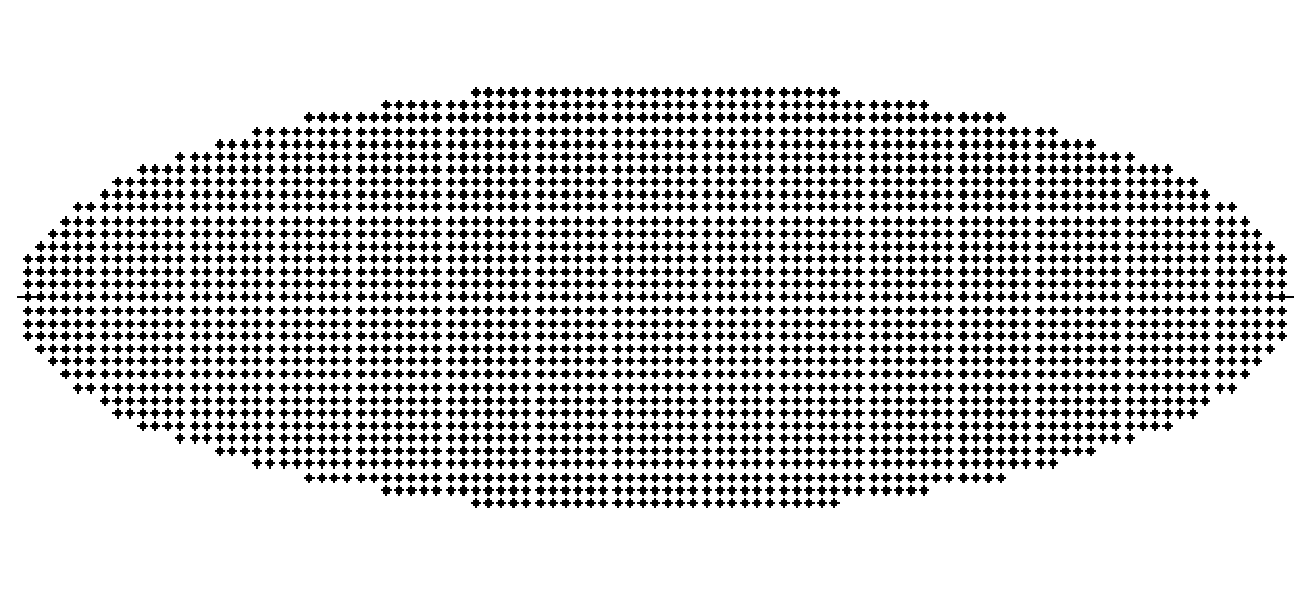
\includegraphics[width=.3\textwidth]{ellipsdot}
\caption{ 3D ellipsoidal cartesian grid is used as model}
\label{fig:ellipsdot}
\end{figure}

The object under study is nanorice,which has an ellipsoid shape. For an initial model of nanorice we assumed an ellipsoid on a 3D cartesian grid in real space. We took the electron density of the nanorice particle to be 1 inside and zero outside the ellipsoid. This model is shown on Figure \ref{fig:ellipsdot} . Subsequently random angle diffraction patterns can be simulated.

The first step of simulation by calculating the structure factor. The structure factor is calculated in reciprocal space using the Fourier transform of the model. The calculation of structure factor and the intensity is
\begin{eqnarray}
A(\hat{q}) &=& \sum_{j} \rho (\hat{r}_{j}) \exp(2 \pi \hat{q}.\hat{r}_{j}) \\
I(\hat{q})&=&|A(\hat{q})|^2. 
\end{eqnarray}
After the intensity is obtained, its spherical harmonics expansion are calculated by integrating the intensity times spherical harmonics over all angles on surface area. Mathematically, the calculation is expressed as 
\begin{eqnarray}
I_{lm}(q) = \int I(q,\theta,\phi) Y_{lm}^{*}(\theta,\phi) d\Omega. 
\label{Ilm}
\end{eqnarray}
Now, random rotation of $I_{lm}$ is performed by multiplying the $I_{lm}$ by rotation matrix. The rotation matrix that has spherical harmonics as their basis functions is Wigner D-matrix. The result of multiplication of the $I_{lm}$ by Wigner D-matrix is new $I_{lm}$ with rotated axes described as  
\begin{eqnarray}
I'_{lm}(q) &=&D^{l}_{m,m'}(\alpha,\beta,\gamma) I_{lm'}^{}(\theta,\phi). \\
\label{IlmD}
\end{eqnarray}

Finally, the diffraction pattern is calculated by slicing the diffraction volume through plane $q_z$=0:
\begin{eqnarray}
I'(q,\theta=\frac{\pi}{2},\phi)&=& \sum_{lm} I'_{lm}(q) Y_{lm}^{}(\theta=\frac{\pi}{2},\phi). 
\end{eqnarray}
This represents the diffraction patterns from random orientations of an nanorice particle. Typical such diffraction patterns are shown in Fig. \ref{fig:dpnano}
\begin{figure}[h]
\begin{subfigure}{.5\textwidth}
  \centering
  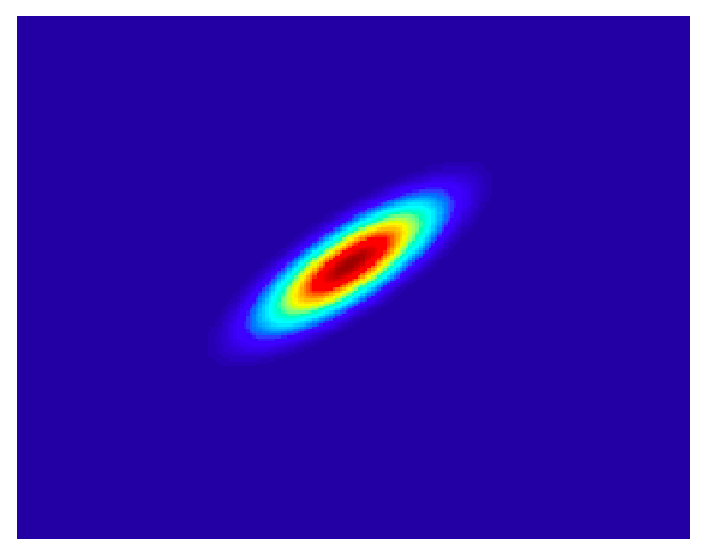
\includegraphics[width=.5\textwidth]{dpnano1}
\end{subfigure}
\begin{subfigure}{.5\textwidth}
  \centering
  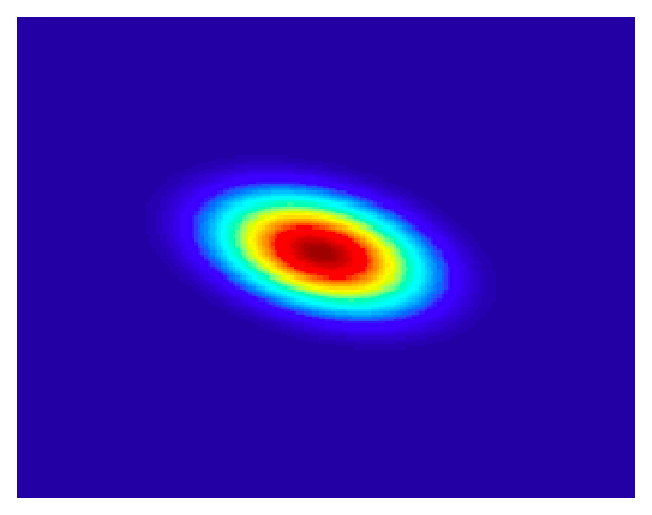
\includegraphics[width=.5\textwidth]{dpnano2}
\end{subfigure}
\caption{Diffraction patterns of nanorice in random orientation}
\label{fig:dpnano}
\end{figure}

Having thus simulated the random orientations diffraction patterns, our next step was to demonstrate it is possible to reconstruct our model of nanorice from those patterns. To do this we have to calculate $B_{l}(q,q)$ and $T_{l}(q,q)$ from the simulated diffraction patterns.

The coefficients of a spherical harmonic expansion ($I_{lm}$) of the diffraction volume clearly depends on the orientation of the diffraction volume relative to the chosen z-axis. Two such 3D intensity distributions are displayed on Fig. \ref{axisno} and Fig, \ref{axisz}. By choosing z-axis at the center of azimuthal symmetry, we eliminate the other components of $I_{lm}$ except m=0.

This suggests some arbitrariness in the reconstruction of the diffraction volume from the measured $B_l$ and $T_l$ coefficients, which are orientation-independent quantities. The quantities $B_l$ and $T_l$ depend on the angular momentum quantum number $l$ but not on the azimuthal quantum number $m$. Yet, in general the spherical harmonic expansion coefficients $I_{lm}(q)$ depend on both sets of quantum numbers. However there is one orientation when the $I_{lm}$ coefficients themselves only depend on $l$, and that is when a major axis of the ellipsoid representing the nanorice is coincident with the z-axis. Under these conditions the particle, and also the diffraction volume has azimuthal symmetry about the z-axis, and can be characterized exactly by $m=0$ for all $l$.

\begin{figure}[h]
\centering
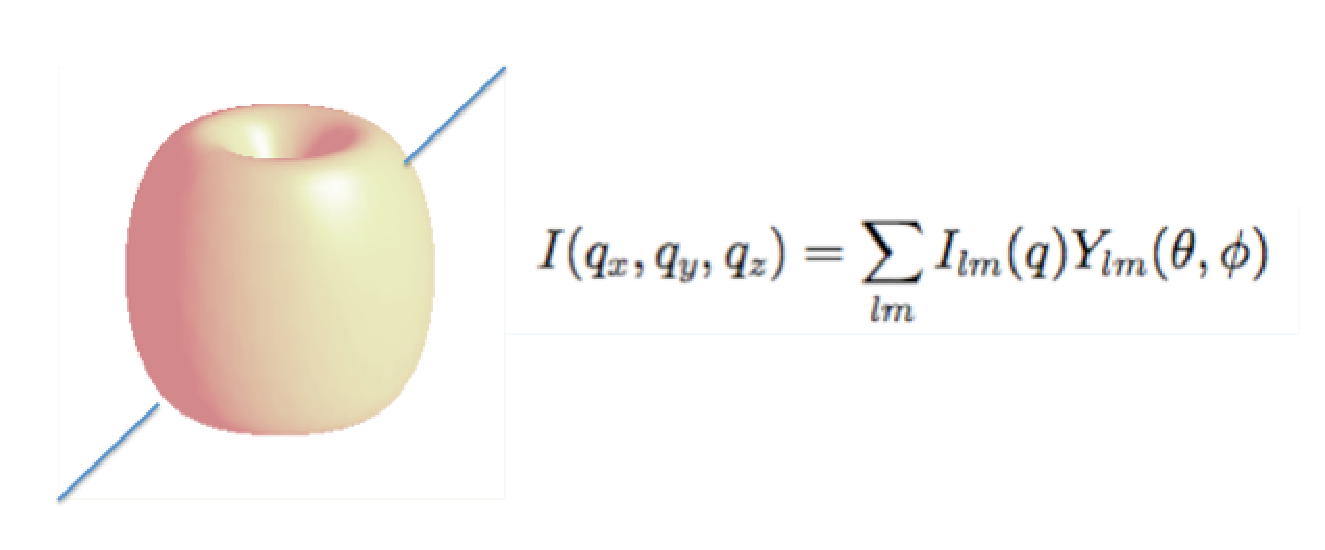
\includegraphics[scale=0.3]{axisno.eps}
\caption{Expansion in spherical harmonics with respect to an arbitrary axis}
\label{axisno}
\end{figure}

\begin{figure}[h]
\centering
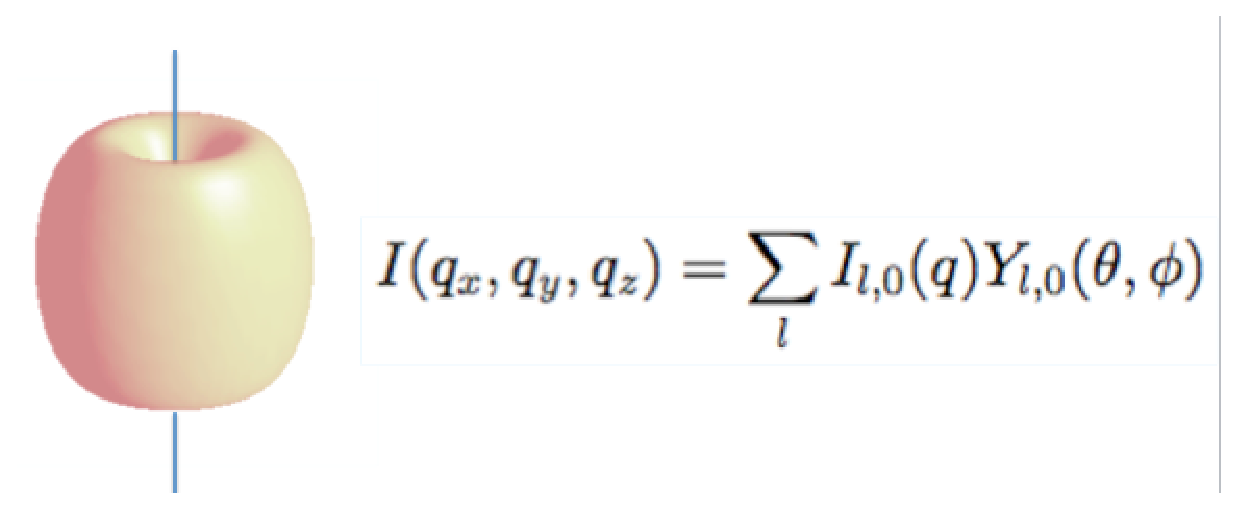
\includegraphics[scale=0.3]{axisz.eps}
\caption{Expansion in spherical harmonics with respect to the z-axis}
\label{axisz}
\end{figure}

We are not trying to reconstruct the particle in any particular orientation. An orientation with the major axis of the ellipsoid along the z-axis is just as good as any other. We can choose this orientation by assuming that only the $m=0$ components of the $I_{lm}(q)$'s exist. At this point these coefficients depend only on $l$, since we assume we know the value of $m$, and we can write

\begin{equation}
|I_{l0}(q)|=\sqrt{B_l(q,q)}. 
\end{equation}

Also, as it is the angular average of the diffraction intensity on a resolution shell of radius $q$, it is a real quantity. Consequently the only ambiguity in $I_{l0}(q)$ is in its sign. We can determine this sign from the triple correlations, since nanorice has azimuthal symmetry. In this case, $m_1=m_2=0$, and the triple correlation reduces to
\begin{equation}
T_l(q,q)=\sum_{l_ll_2} I_{l0}(q) I_{l_10}(q) I_{l_20}(q) G(l0; l_10; l_20)
\label{tsimp}
\end{equation}
where $G$ is a Gaunt coefficient \cite{pendry1974}.

Since an ellipsoid has azimuthal symmetry at particular axis, we can choose that particular axis as z-axis, thus eliminating any other components of $I_{lm}$ except $m=0$. $|I_{l,0}|$ can be obtained directly from $B_{l}$ via
\begin{eqnarray}
|I_{l,0}(q)|=\sqrt{B_{l}(q)}.
\label{Il0B}
\end{eqnarray}
The only unknown here is sign of $I_{l,0}$. The sign can be determined by fitting all possible signs of $I_{l,0}$ to the "experimental" triple correlations in (\ref{tsimp}).

After obtaining the signs of the $I_{l.0}$, the diffraction volume can be calculated from
\begin{eqnarray}
I(\hat{q})=\sum_{l,0} I_{l,0} Y_{l,0}(\theta,\phi). 
\end{eqnarray}

To test the method, 200 random angle diffraction patterns were simulated. Typical diffraction patterns are shown in figure \ref{fig:dpnano}.  After simulating the diffraction patterns, they were used as the input to calculate $C_{2}$, $C_{3}$, $T_{l}(q)$ and $B_{l}(q,q)$. For the reconstruction, the parameter $l_{max}=16$ was used as a cut off of the maximum value for $l$.  

As explained above, by knowing $B_{l}(q)$ and $T_{l}(q)$, the diffraction volume can be found after constraining their spherical harmonics expansion to be nonzero when $m=0$. An iterative phasing algorithm \cite{oszlanyi2004, oszlanyi2005} applied to this diffraction volume could then recover the electron density. The reconstructed electron density after phasing is displayed in figure \ref{fig:rhoflat}. Figure \ref{fig:rhoflat} shows that the method can reconstruct the original ellipsoid model from a set of random angle diffraction pattern. 

\begin{figure}[h!]
\centering
 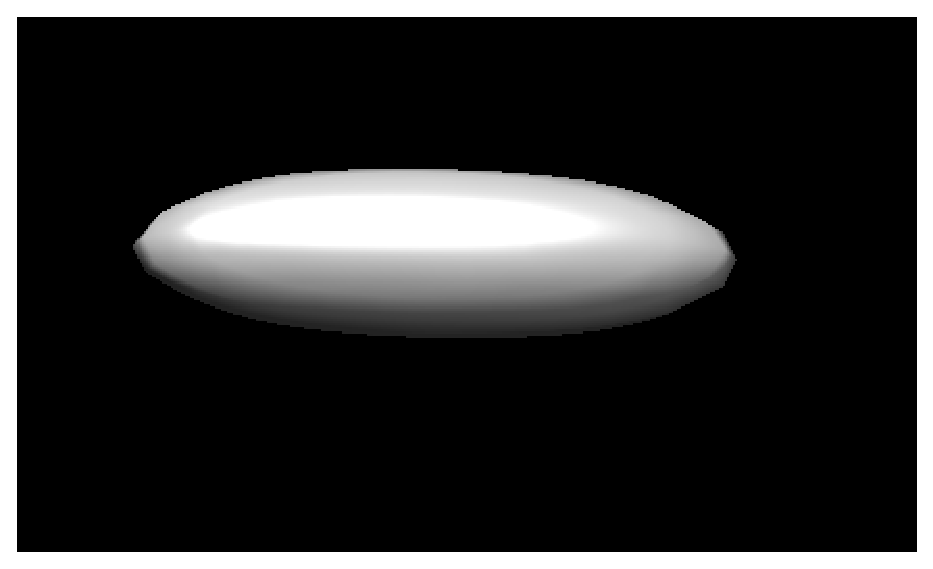
\includegraphics[width=.4\textwidth]{rhoflat}
\caption{Reconstructed electron density after phasing}
\label{fig:rhoflat}
\end{figure}

Another test of this method was by calculating $R_{split}$. A sets of diffraction patterns were simulated and they were splitted into two sets of diffraction patterns (each set has 200 patterns). By having 2 sets, now there were 2 different quanities for $C_{2}$, $C_{3}$, $B_{l}(q)$, and $T_{l}(q)$. Each quantities was used to calculate two different diffraction volumes. After getting two different diffraction volumes, formula for $ R_{split} $ was used as follow:

\begin{align}
R_{split}(q)=\frac{1}{2^{1/2}}\frac{\sum_{|q|} |I_{1} - I_{2}|}{\frac{1}{2} \sum_{|q|}(I_{1}+I_{2})} 
\end{align} 
where the summation is performed over all point in shell surface with the same value of $q$. 

\begin{figure}[h!]
\centering
 \includegraphics[width=.5\textwidth]{Rsplit}
\caption{Plot of $R_{split}$ vs $q$}
\label{fig:Rsplit}
\end{figure}

The quantity $q_{max}$ can be estimated using 
\begin{align}
q_{max}=\frac{l_{max}}{2 \pi R}
\label{eq:qmaxlmax}
\end{align}
where $l_{max}=16$ and $R=25$ Ang. By using equation \ref{eq:qmaxlmax}, it is expected that the $q_{max}$ is accurate until $0.1$ Ang$^{-1}$. In figure \ref{fig:Rsplit}, it is shown that the $R_{split}$ is reasonable enough when $q_{max}$ is less than $0.1$ Ang$^{-1}$ and $R_{split}$ goes higher after $q_{qmax}=0.1$ Ang$^{-1}$.  

Beside $R_{split}$, Fourier shell correlation (FSC) was used to characterize the reconstruction. As explained above, $R_{split}$ do the comparison of two diffraction volumes before they are used in phasing. In constrast to $R_{split}$, FSC includes the comparison of the reconstruction after phasing. Thus, the two diffraction volumes from earlier calculation were used as the inputs of the phasing and the outputs of it were the two different electron densities. 

The eletron densities from phasing algorithm have arbitrary center. Before calculating FSC, the centering was performed by finding the location of a box, which has largest value of the electron density. After getting the location of the box, the center of the box was taken as the center of the electron density. Subsequent to that, two structure factors were calculated by performing Fourier transform of the electron density. Following to that, FSC can be calculated using the following formula
\begin{align}
FSC(q)=\frac{\sum_{|q|} F_{1}(q) F_{2}(q)^{*}}{\sqrt{\sum_{|q|}|F_{1}(q)|^2}\sqrt{\sum_{|q|}|F_{2}(q)|^2}}
\label{eq:FSC}
\end{align}
where the summation is performed over all point in shell surface with the same value of $q$. 
\begin{figure}[h!]
\centering
 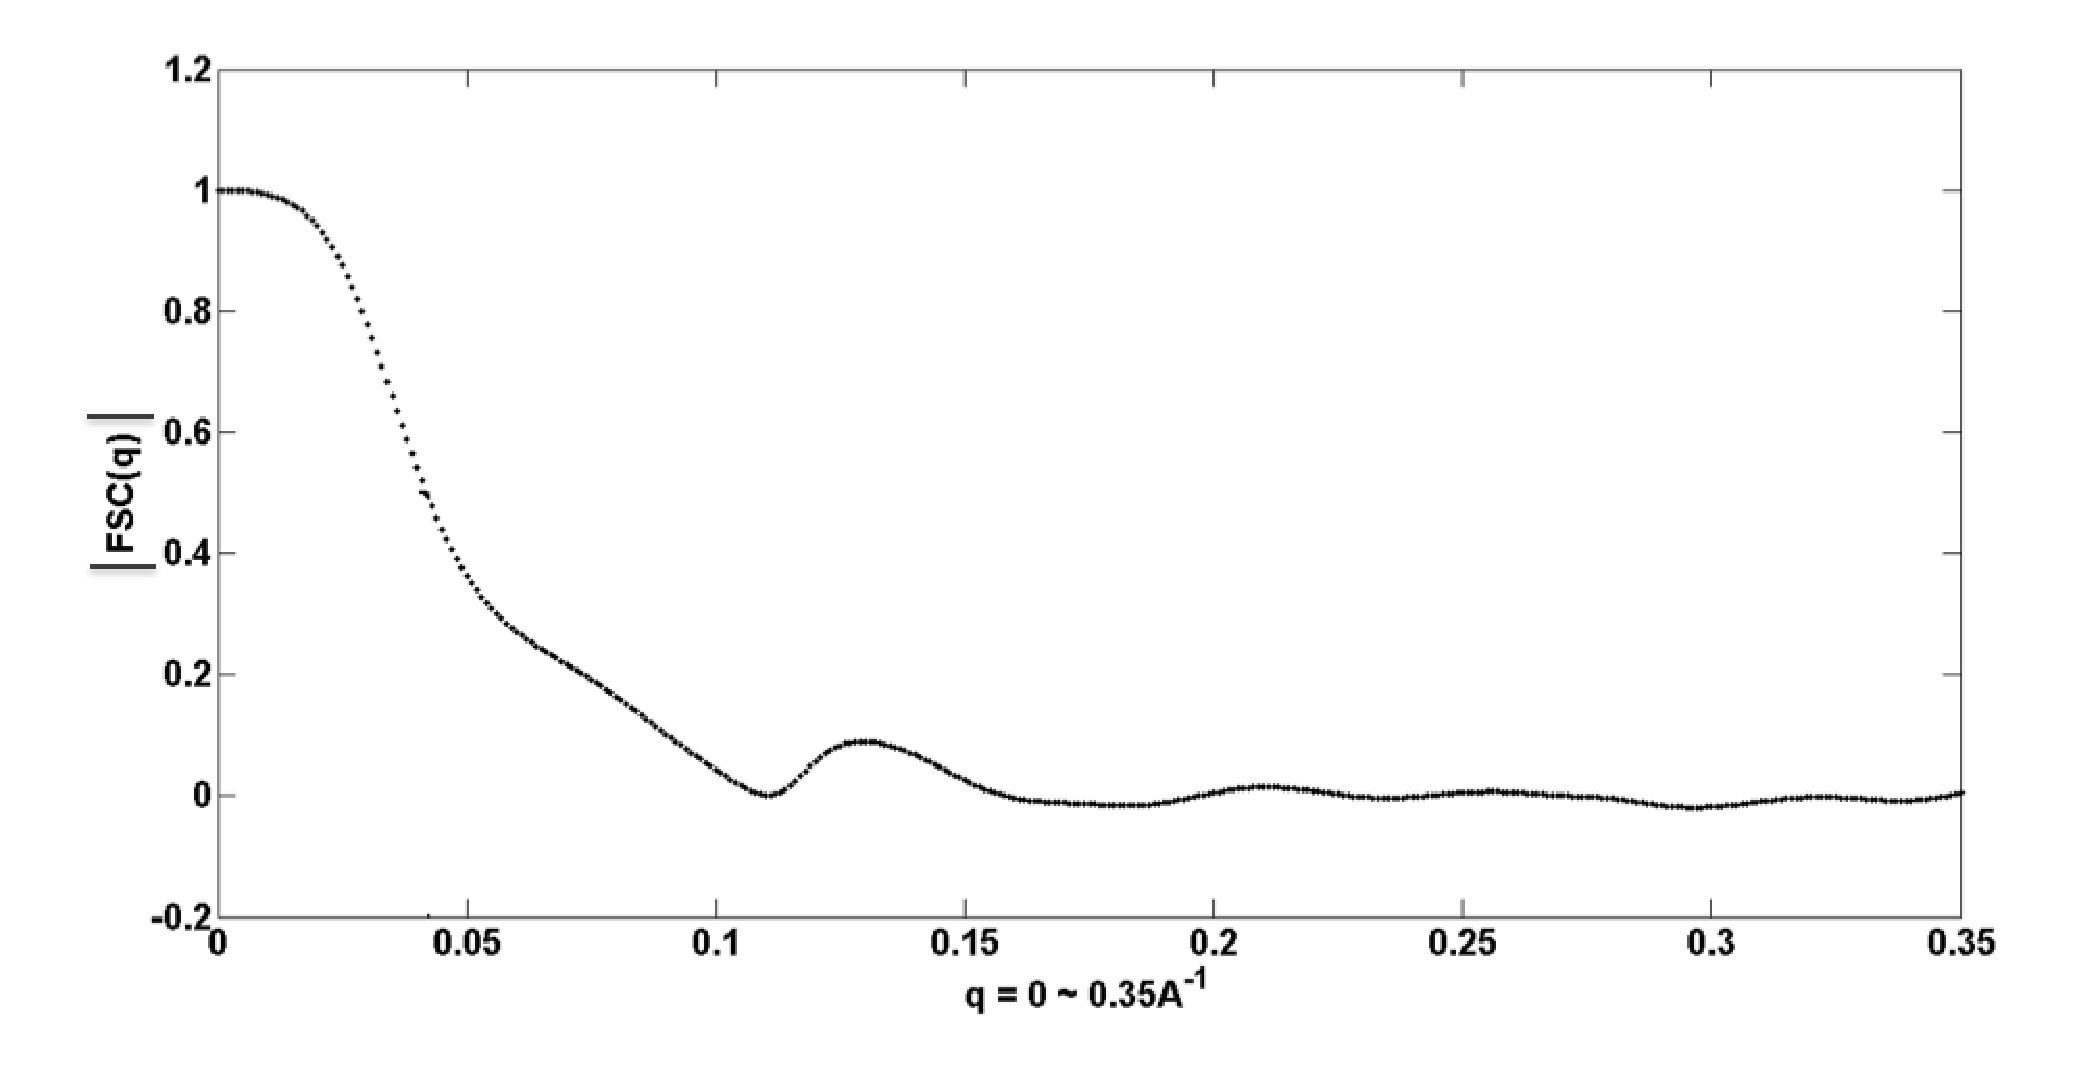
\includegraphics[width=.9\textwidth]{FSC}
\caption{Plot of modulus of FSC vs $q$ }
\label{fig:FSC}
\end{figure}

Figure \ref{fig:FSC} shows the plot of the modulus of FSC vs $q$. The FSC goes down as $q$ goes higher. The graph shows that even though $q_{max}=0.1$, the actual accuracy for $q_{max}$ is lower than that. If $0.5$ is taken as the limit of acceptable value of FSC then the actual $q_{max}$ is around $0.05$. Many factor can contribute to the calculation of FSC such as the total number of the diffraction patterns, the phasing algorithm, and the process of centering the electron density. 

%To further test the method, another more complicated azimuthal shape was tested. The diffraction patterns from the shape displayed in figure \ref{fig:orbitmod} was simulated. Subsequently the \Blq were calculated and the signs can be determined from $T_{l}(q,q)$. After phasing the reconstruction is displayed in figure \ref{fig:orbitrec}.  

%\begin{figure}[h!]
%\begin{subfigure}{.5\textwidth}
  %\centering
  %\includegraphics[width=.3\textwidth]{orbit1}
%\end{subfigure}
%\begin{subfigure}{.5\textwidth}
  %\centering
  %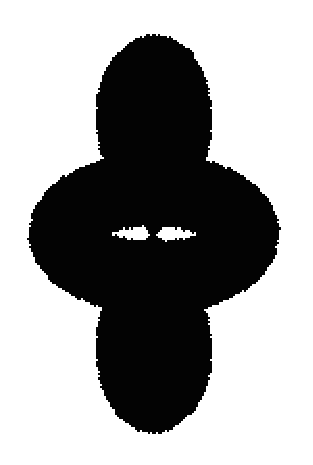
\includegraphics[width=.3\textwidth]{orbit2}
%\end{subfigure}
%\caption{Azimuthal model }
%\label{fig:orbitmod}
%\end{figure}
%\begin{figure}[h!]
  %\centering
  %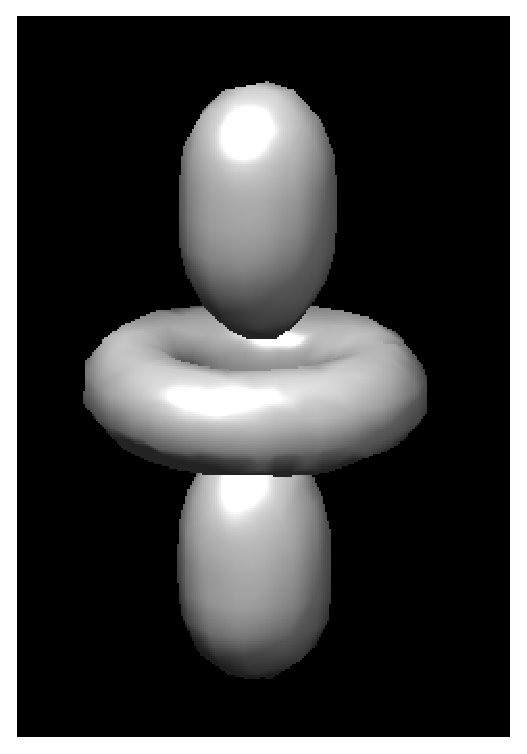
\includegraphics[width=.3\textwidth]{orbitrec}
%\caption{Reconstruction from \Blq }
%\label{fig:orbitrec}
%\end{figure}

%In this section, it is demonstrated how the electron density is reconstructed from a collection of random diffraction patterns and the final reconstruction is able to reproduce its original model.  

